% Template LaTeX file for DAFx-11 papers

%------------------------------------------------------------------------------------------
%  !  !  !  !  !  !  !  !  !  !  !  ! user defined variables  !  !  !  !  !  !  !  !  !  !  !  !  !  !
% Please use these commands to define title and author of the paper:
\def\papertitle{FAUST-STK: a set of linear and nonlinear physical
  models for the FAUST programing language}
\def\paperauthorA{Romain Michon}
\def\paperauthorB{Julius O. Smith}


%------------------------------------------------------------------------------------------
\documentclass[twoside,a4paper]{article}
\usepackage{dafx_11}
\usepackage{amsmath,amssymb,amsfonts,amsthm}
\usepackage{euscript}
\usepackage[latin1]{inputenc}
\usepackage[T1]{fontenc}
\usepackage{ifpdf}

\usepackage[english]{babel}
\usepackage{caption}
\usepackage{subfig, color}

\setcounter{page}{1}
\ninept

\usepackage{times}
% Saves a lot of ouptut space in PDF... after conversion with the distiller
% Delete if you cannot get PS fonts working on your system.

% pdf-tex settings: detect automatically if run by latex or pdflatex
\newif\ifpdf
\ifx\pdfoutput\relax
\else
   \ifcase\pdfoutput
      \pdffalse
   \else
      \pdftrue
\fi

\ifpdf % compiling with pdflatex
  \usepackage[pdftex,
    pdftitle={\papertitle},
    pdfauthor={\paperauthorA},
    colorlinks=false, % links are activated as colror boxes instead of color text
    bookmarksnumbered, % use section numbers with bookmarks
    pdfstartview=XYZ % start with zoom=100% instead of full screen; especially useful if working with a big screen :-)
  ]{hyperref}
  \pdfcompresslevel=9
  \usepackage[pdftex]{graphicx}
  \usepackage[figure,table]{hypcap}
\else % compiling with latex
  \usepackage[dvips]{epsfig,graphicx}
  \usepackage[dvips,
    colorlinks=false, % no color links
    bookmarksnumbered, % use section numbers with bookmarks
    pdfstartview=XYZ % start with zoom=100% instead of full screen
  ]{hyperref}
  % hyperrefs are active in the pdf file after conversion
  \usepackage[figure,table]{hypcap}
\fi

\title{\papertitle}


\twoaffiliations{
\paperauthorA,\sthanks{CCRMA visiting researcher from Saint \'Etienne
  University, France. Work carried out in the frame of the ASTREE
  Project (ANR-08-CORD-003).}}
{\href{http://ccrma.stanford.edu/~rmichon}{CIEREC, EA 3068} \\ Universit� Jean
  Monnet \\ F-42023, Saint-Etienne, France \\
{\tt \href{mailto:rmichon@ccrma.stanford.edu}{rmichon@ccrma.stanford.edu}}
}
{\paperauthorB,}
{\href{https://ccrma.stanford.edu/\~{}jos/}{Center for Computer Research in Music and Acoustics.}\\ (CCRMA) Stanford University \\ Palo Alto, CA 94305, USA\\
{\tt \href{mailto:jos@ccrma.stanford.edu}{jos@ccrma.stanford.edu}}
}


\begin{document}
% more pdf-tex settings:
\ifpdf % used graphic file format for pdflatex
  \DeclareGraphicsExtensions{.png,.jpg,.pdf}
\else  % used graphic file format for latex
  \DeclareGraphicsExtensions{.eps}
\fi

\maketitle

\begin{abstract}

The {\it FAUST Synthesis ToolKit} is a set of virtual musical
instruments written in the FAUST programming language and
based on waveguide algorithms and on modal synthesis. Most of them
were inspired by instruments implemented in the {\it Synthesis
  ToolKit} and the program {\it SynthBuilder}.

Our attention has partly been focused on the pedagogical aspect of the implemented
objects. Indeed, we tried to make the FAUST code of each objects as optimized and
as expressive as possible.

Some of the instruments in the {\it FAUST-STK} use nonlinear allpass
filters to create interesting and new behaviors. Also, a few
of them were modified in order to use following gesture datas to
control the performance. A demonstration of this kind of use is done
in the {\it PureData} program.

Finally, the results of some performances tests of the generated C++
code are presented.   

\end{abstract}

\section{Introduction}\label{sec:intro}

The {\it FAUST Synthesis ToolKit} is set of virtual musical instruments
programmed in the FAUST\footnote{Functional AUdio STream is programming language that
  proposes an abstract, purely functional approach to signal
  processing. It has been developed at Lyon's GRAME (Groupe de
  recherche en Acoustique et en Musique Electronique) since 2002:
  \url{http://faust.grame.fr/}.} programing language. Most of them are
based on physical models inspired from the algorithms implemented in the {\it Synthesis
  ToolKit (STK)} \cite{STK} and the program {\it SynthBuilder}
\cite{synthBuilder}.

The {\it STK} is developed since 1996 by P. R. Cook and
G. P. Scavone. It is a set of open source audio signal processing and
algorithmic synthesis classes written in the C++ programming
language that can be used in the development of music synthesis and
audio processing
software\footnote{\url{https://ccrma.stanford.edu/software/stk/}.}.

In the other hand, {\it SynthBuilder} was a program used at Stanford's
CCRMA\footnote{Center for Computer Research in Music and Acoustics} in
the nineties to implement physical models of musical instruments. Most
of its algorithms use the waveguide synthesis technique but some of
them are also based on modal synthesis. 

An important part of our work consisted at improving and simplifying
the models from these two sources in order to make them more efficient
thanks to the FAUST semantic. All the FAUST codes from the {\it
  FAUST-STK} are commented and refer as often as possible to external
bibliographical elements. Finally, lots of the algorithms from the {\it STK} and {\it
  SynthBuilder} were upgraded with nonlinear allpass filters.

First, we will present the different models of musical instruments implemented in the {\it
  FAUST-STK}. We will discuss about the problems we encountered
during their development and then describe the selected solutions. A
brief overview on the use of allpass nonlinear filters with waveguide
models will be done. Finally, we'll study the performances of the
generated C++ code.    

\section{Waveguide Models}\label{sec:waveguideModels}

Waveguide synthesis was created by J. O. Smith during the
eighties \cite{waveGuide}. It is based on a modified version of the
Karplus-Strong algorithm \cite{KS} that makes it possible to model any
kind of string, bore or vibrating structures with a network of delay
lines and filters. Waveguide instruments appears to be very suitable to be implemented with
the FAUST language mainly because of their ``stream like''
architecture.   

A brief overview of the {\it FAUST-STK} waveguide instruments is done in this section.

\subsection{Wind Instruments}

The algorithms used in the {\it FAUST-STK} are almost all based on
instruments implemented in the {\it Synthesis ToolKit} and the program
{\it SynthBuilder}. Although, it is important to observe that some of
them were slightly modified in order to adapt them to the FAUST semantic.

Despite the fact that we used as often as possible functions already
defined in the default FAUST libraries to build our models, we needed
most of the time to write our own filters in order to be able to use the
parameters from the {\it STK} classes and the {\it SynthBuilder}
patches. All these functions were put in a file called
\texttt{instrument.lib}.

All the wind instruments implemented in the {\it FAUST-STK} are based
on a similar architecture. Indeed, in most cases, the breath pressure
that correspond to the amplitude of the excitation is controlled by an
envelope. The excitation is used to feed one or several waveguides that
implements the body of the instrument. For example, in the case of a
clarinet, the excitation corresponds to the reed that vibrates in the
mouthpiece and the body of the instrument is the bore and the bell. 
In figure \ref{fig:clarinet}, it is possible to see the block diagram
of one of the two clarinet models that are implemented in the {\it
  FAUST-STK}. In that case, an ADSR\footnote{Attack - Decay - Sustain -
  Release.} envelope that is embedded in the {\it breathPressure} box
controls the breath pressure.

The other clarinet implemented in the {\it FAUST-STK} is a bit
  more complex as it has a tone hole model that makes it possible
  to change the pitch of the note being played in a more natural
  way. Indeed, in the algorithm showed in figure \ref{fig:clarinet}
  and as in most of the basic waveguide models,
  the pitch is modulated by changing the length of the loop delay line
  which would correspond in ``the real world'' to changing dynamically
  the size of the clarinet's bore during the performance which is of
  course impossible.    

\begin{figure}[ht]
\begin{center}
        \framebox{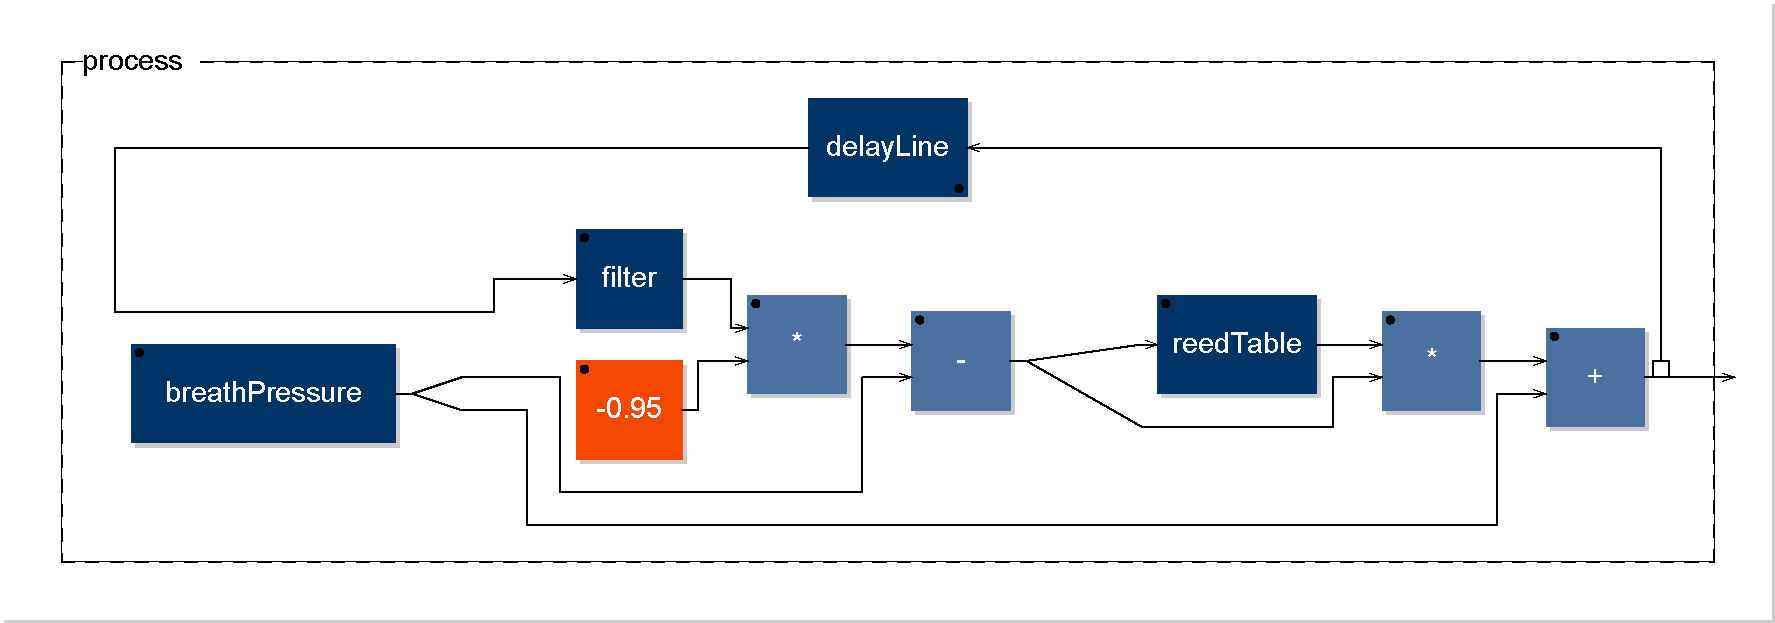
\includegraphics[width=\columnwidth]{fig/clarinet.pdf}}
\caption{{\it \texttt{clarinet.dsp} algorithm drawn by FAUST using faust2pd.}}
\label{fig:clarinet}
\end{center}
\end{figure}

The reed table employed with the two clarinets to excite the model was
also used to create a very simple saxophone model that is even more
comparable to a violin whose strings are excited by a reed.   

Two models of flute are implemented in the {\it FAUST-STK}. The first one
is based on the algorithm used in the {\it Synthesis ToolKit} that is a
simplified version of \cite{jet}. The other model is showed in figure
\ref{fig:flute}. It uses two loops
and a more sophisticated jet filter (a butterworth filter is used instead of
a simple one pole).    

\begin{figure}[ht]
\begin{center}
        \framebox{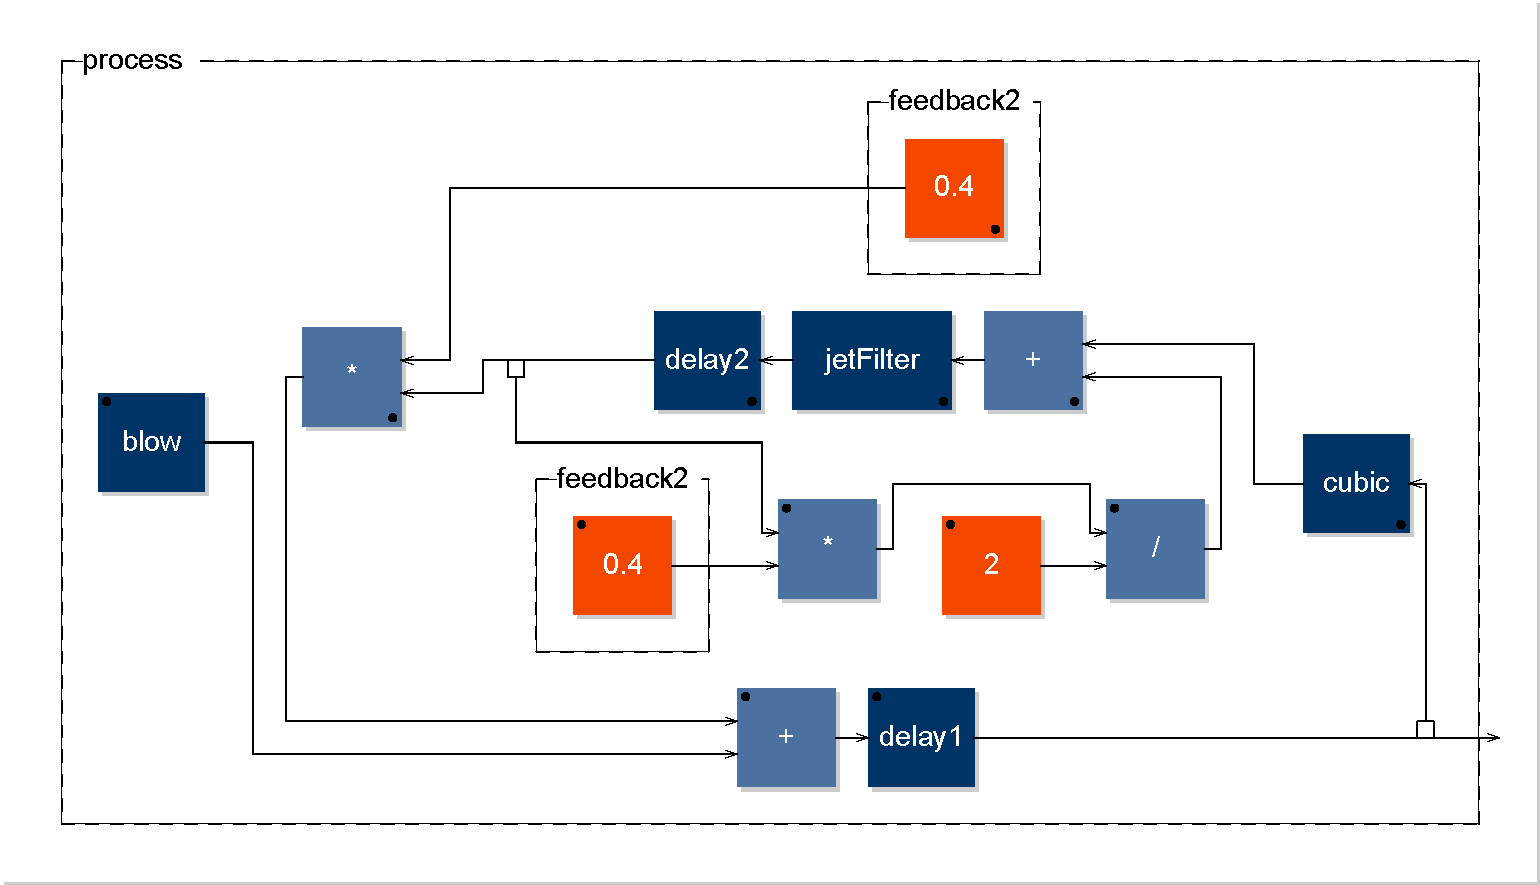
\includegraphics[width=\columnwidth]{fig/flute.pdf}}
\caption{{\it \texttt{flute.dsp} algorithm drawn by FAUST using faust2pd.}}
\label{fig:flute}
\end{center}
\end{figure}

A simple model of a brass instrument inspired from a class of the {\it Synthesis
  ToolKit} and with a mouthpiece based on the model described in
\cite{brassMouth} is implemented in the {\it FAUST-STK}. It can be used to
emulate a wide range of instrument such as a french horn, a
trumpet or even a trombon. Its algorithm can be seen in figure \ref{fig:brass}.  

\begin{figure*}[ht]
\begin{center}
        \framebox{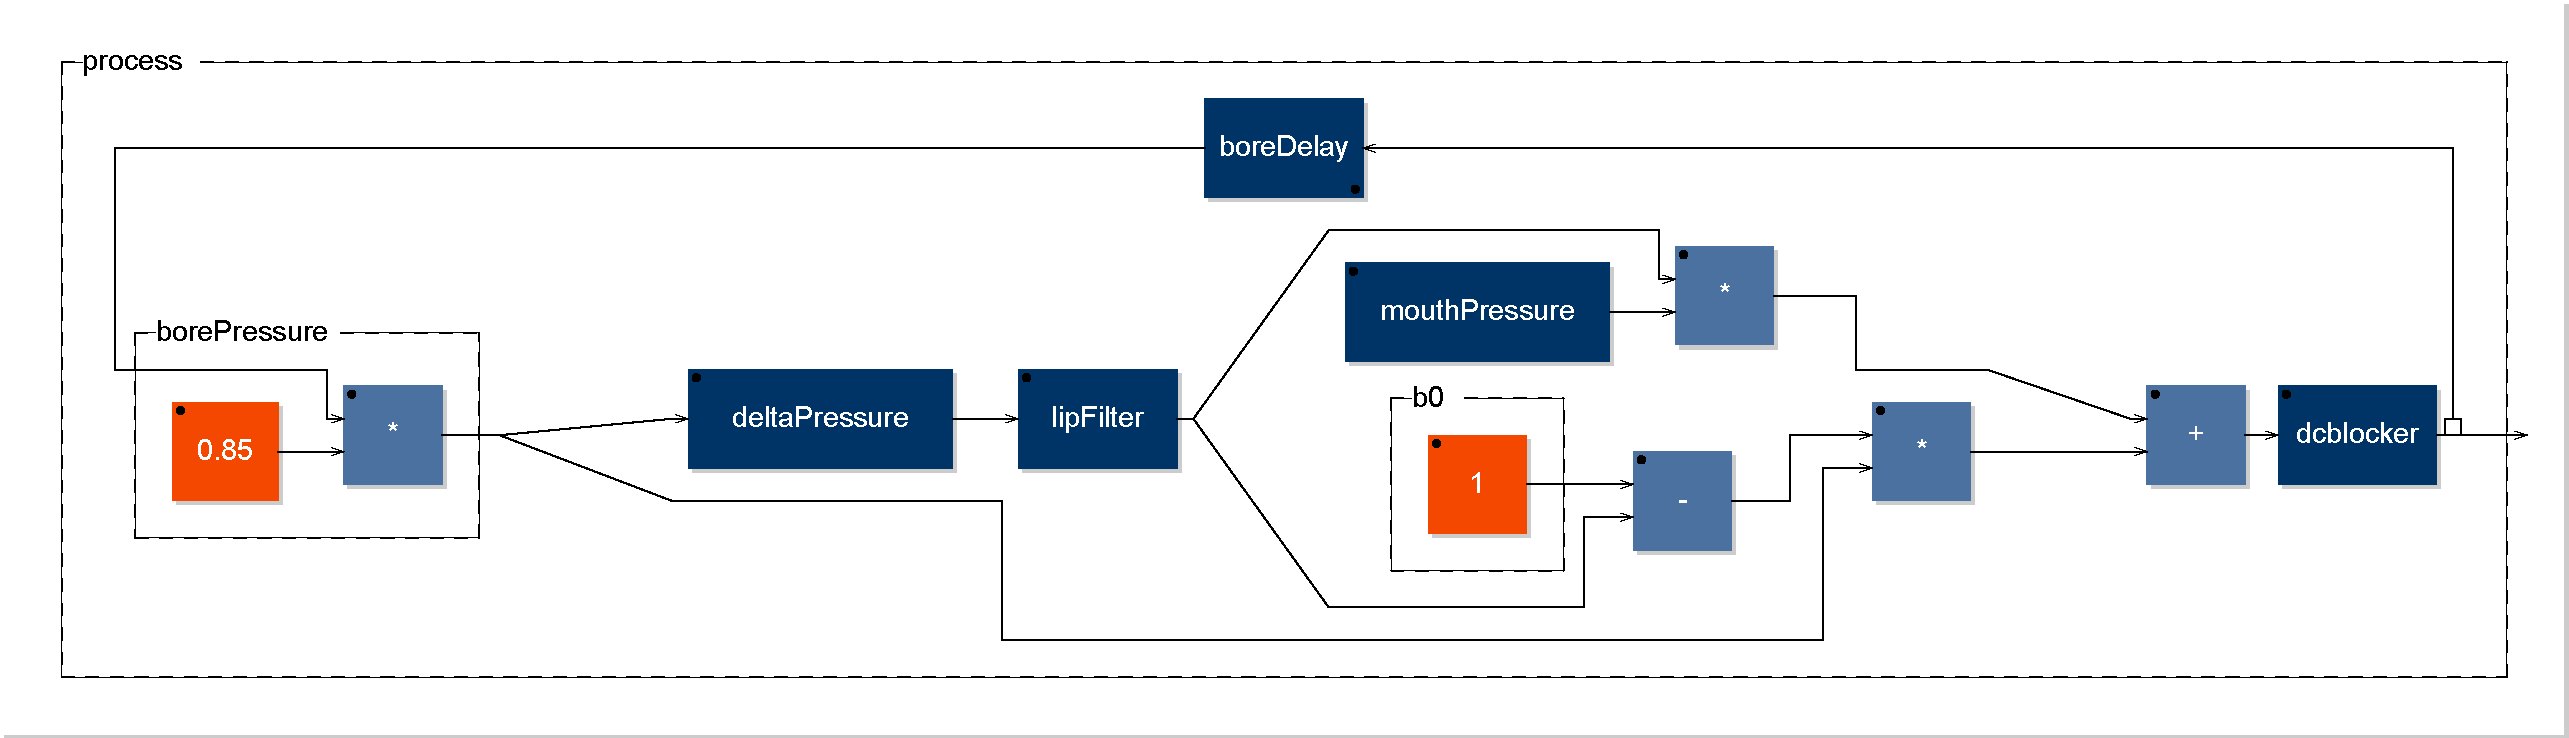
\includegraphics[width=\textwidth]{fig/brass.pdf}}
\caption{{\it \texttt{brass.dsp} algorithm drawn by FAUST using faust2pd.}}
\label{fig:brass}
\end{center}
\end{figure*}

Finally, a tuned bottle where it is possible to blow through the neck
to make sound is also implemented in the {\it FAUST-STK}.

\subsection{String Instruments}\label{subsec:strings}

Some of the waveguide algorithms for plucked strings have
already been implemented in FAUST by J. O. Smith that worked in
\cite{faustEks} on the extended Karplus-Strong. Although, it is
possible to find in the {\it FAUST-STK} a few models of string
instruments such as a Sitar, a bowed string instrument, a nonlinear
extended Karplus-Strong (Cf. \ref{sec:NLF} about nonlinear waveguide models), an acoustic bass, a piano and
an harpsichord (Cf. \ref{sec:keyboards} about keyboards instruments in
the {\it FAUST-STK}). 

Except the nonlinear extended Karplus-Strong,
all this algorithms are inspired from the {\it Synthesis ToolKit} and
the program {\it SynthBuilder}.   

\subsection{Percussion Instruments}\label{subsec:drums}

Four objects in the {\it FAUST-STK} use the banded waveguide
synthesis technique (described in \cite{bdWaveGuides}) to model the following percussion instruments:
\begin{itemize}
\item an iron plaque;
\item a wooden plaque;
\item a glass plaque;
\item a tibetan bowl.
\end{itemize}

Each of them can be excited with a bow or a hammer.

\section{Using nonlinear passive allpass filter with waveguide models}\label{sec:NLF}

Some of the instruments implemented in the {\it FAUST-STK} are using
nonlinear passive allpass filters in order to generate nice natural and
unnatural sound effects. 
The allpass Ladder and Latice filters described in \cite{linearSpeech}
makes it possible to create nonlinear behaviors when they are used in
waveguide algorithms. The nonlinearities are generated by
dynamicaly modulating the filter coefficients at every sample. For the
instruments that use this kind of filter in the
{\it FAUST-STK}, the user can decide whether the coefficients are
modulated by the incoming signal or by a sine wave. In both cases, a
``nonlinearity factor'' parameter scale the range of the modulation of the
filter coefficients. This parameter can be controlled by an envelope
in order to make the nonlinear behavior more natural.
  
It is necessary to adjust the length of the delay line of the
instruments that use nonlinear allpass filters in function of the
nonlinearity factor and of the order of the filter as follow:
\begin{equation}
DL = (SR/F) - FO.NF 
\end{equation}
where DL is the delay length in number of samples, SR is the sampling
rate, F is the pitch frequency, FO is the filter order and NF the
nonlinearity factor (value between 0 and 1).

Typically, the nonlinear allpass filter has to be placed just before
the feedback of the waveguide loop as showed in figure \ref{fig:clarinetNL}.

\begin{figure}[ht]
\begin{center}
        \framebox{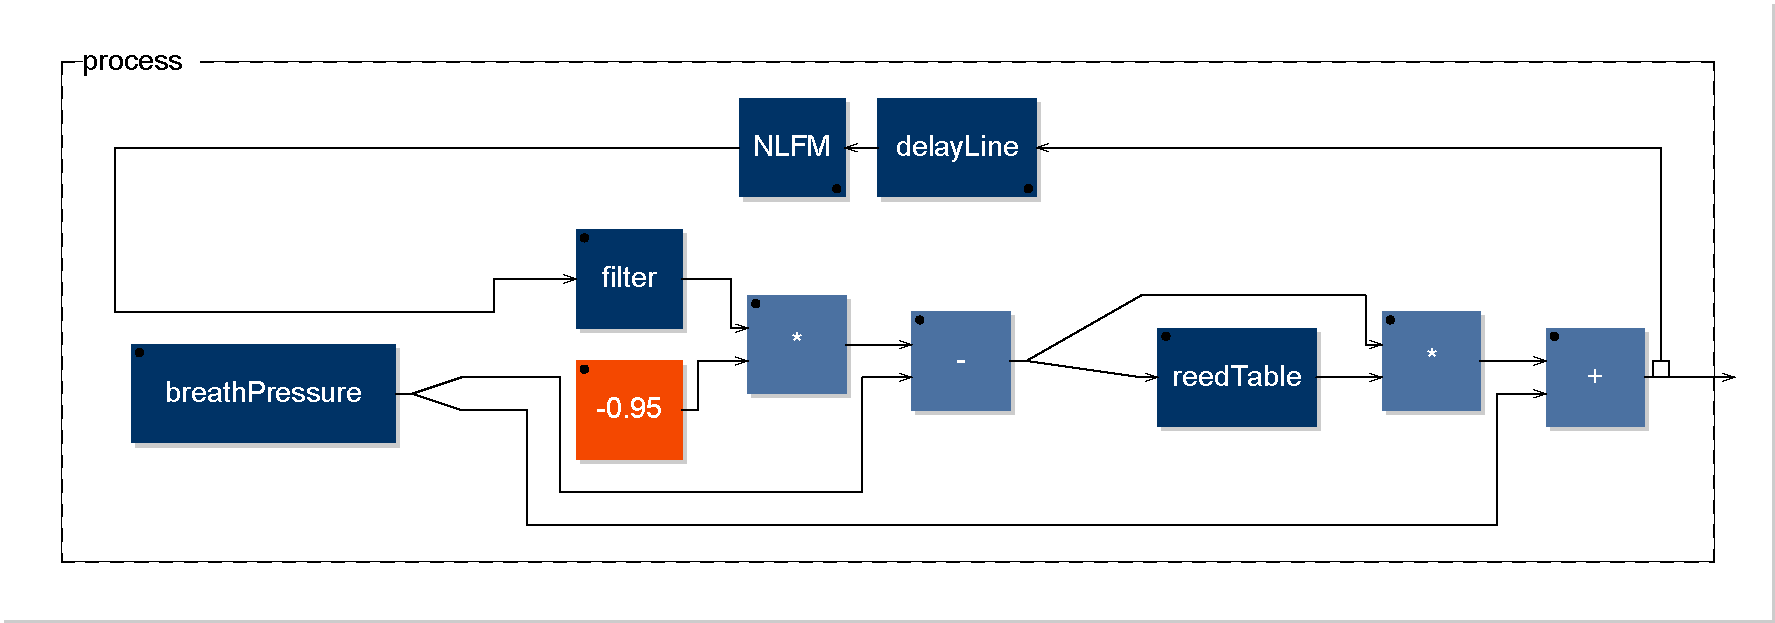
\includegraphics[width=\columnwidth]{fig/clarinetNL.pdf}}
\caption{{\it Modified version of \texttt{clarinet.dsp} (Cf. figure
    \ref{fig:clarinet}) that uses a nonlinear allpass filter in its
    feedback loop.}}
\label{fig:clarinetNL}
\end{center}
\end{figure}

Finally, it is interesting to mention that we were able to implement a
frequency modulation synthesizer in the {\it FAUST-STK} by using this
kind of filter on a sine wave signal. 

\section{Modal Models}\label{sec:modal}

A set of instruments using modal synthesis can be found in the {\it
  FAUST-STK}. They are all implemented in the same code as they are based on the same algorithm.

Modal synthesis was discovered by J-M. Adrien in the eighties \cite{modal} and
is very similar to the technique used in \ref{subsec:drums} as it
consists in exciting a filter bank with an impulsion (figure
\ref{fig:modal}).

Implementing modal synthesis with FAUST was a bit chalenging. Indeed,
it requires to handle an important amount of values and to use an
excitation signal stored in a wave file. The first problem was solved
by using the foreign function primitive in FAUST that allows to use
C++ function within a FAUST code. The different values were stored in
an array of floats used in a function that takes an index as an argument and
that returns the corresponding number.

In order to solve the other problem about importing a wave table in a
FAUST object from a wave file, we first tried to use the
\texttt{libsndfile} library developed by E. de Castro Lopo
\cite{libsndfile} that makes it possible to easily handle wave files
in C++. Unfortunately, it appears that this solution was not
compatible with all the FAUST architectures. Based on this observation
and the fact that the wave tables used in the STK had a maximal size
of 1024 samples, we decided to use
the same technique than the one previously explained. Indeed, the raw
datas were extracted from the wave file to be put in an array of floats that
can be used in a C++ function to return the values with an index. This
C++ function can then be called in FAUST using the foreign function
mechanism to fill a buffer with the \texttt{rdtable} primitive.   

\begin{figure*}[ht]
\begin{center}
        \framebox{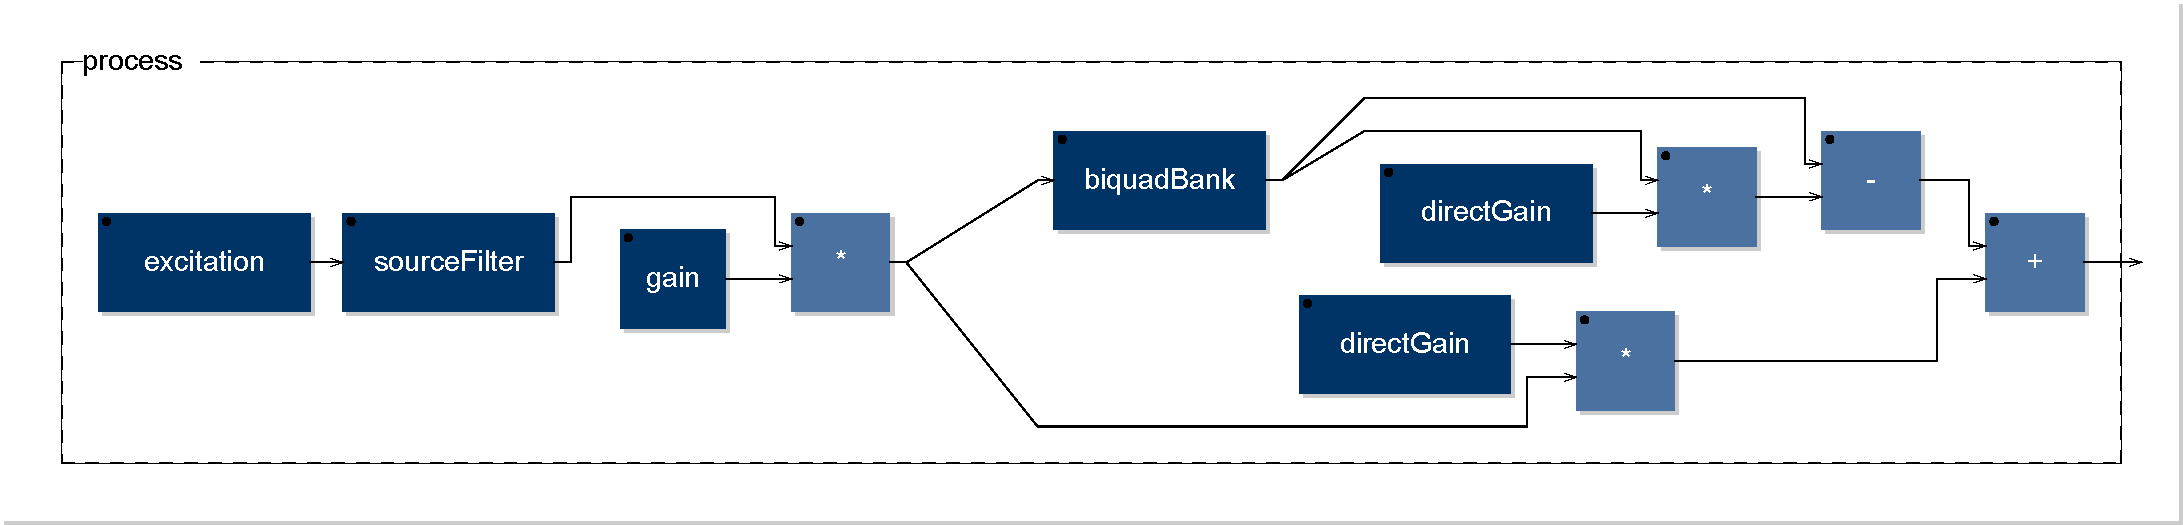
\includegraphics[width=\textwidth]{fig/modalBar.pdf}}
\caption{{\it \texttt{modalBar.dsp} algorithm drawn by FAUST using faust2pd.}}
\label{fig:modal}
\end{center}
\end{figure*}

\section{Voice Synthesis}

A very simple voice synthesizer based on the algorithm from
the {\it Synthesis ToolKit} is implemented in the {\it FAUST-STK}. It
uses a wave table to excite a bank of 4 bandpass filters that shape
the voice formants. The formant values are stored in a C++ function in the
same way than described in \ref{sec:modal} as a set of center
frequencies, amplitudes and bandwidths. This function is then called
in the FAUST code using the foreign function primitive. The thirty-two
phonemes stored in this function are the same than the one from the
{\it Synthesis ToolKit}. 

\section{Keyboards}\label{sec:keyboards}

A {\it SynthBuilder} patch implementing a commuted piano \cite{commutedPiano} has been
written in the late nineties at Stanford's CCRMA. This patch was partly
ported in 2006 by Stephen Sinclair at McGill University in the {\it
  Synthesis ToolKit} \cite{pianoSTK}. A big part of his work consisted
in extracting the values for each parameters from the {\it
  SynthBuilder} patch to store them in a set of C++ functions. We
reused them to build our FAUST commuted piano version by using the
{\it foreign function} mechanism as described in \ref{sec:modal}.

In this piano model, the keyboard is splited in two part which use a
different algorithm. Indeed, the tones
below {\it E6} use the commuted waveguide technique while tones above
or equal to {\it E6} use a serie of biquad filters to generate the
sound (figure \ref{fig:piano}).   

\begin{figure}[ht]
\begin{center}
        \framebox{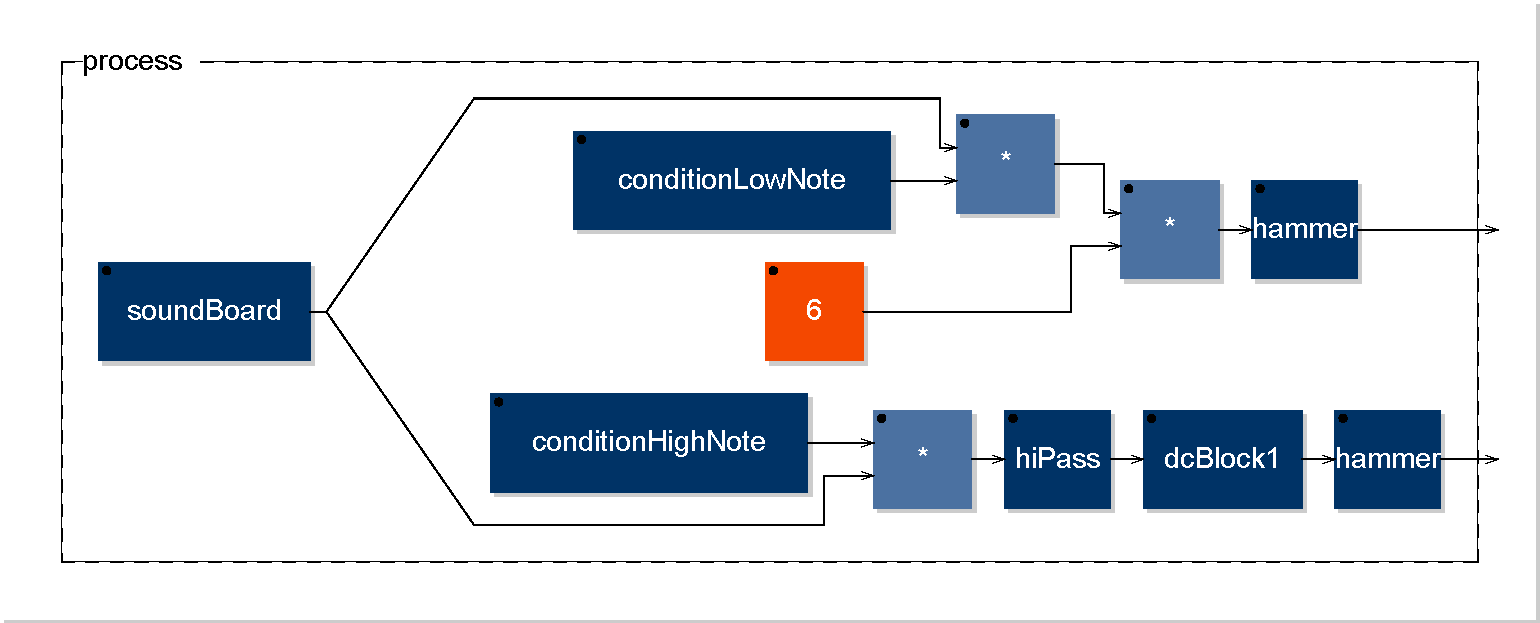
\includegraphics[width=\columnwidth]{fig/piano1.pdf}} \\
        \hspace{2cm}
        \framebox{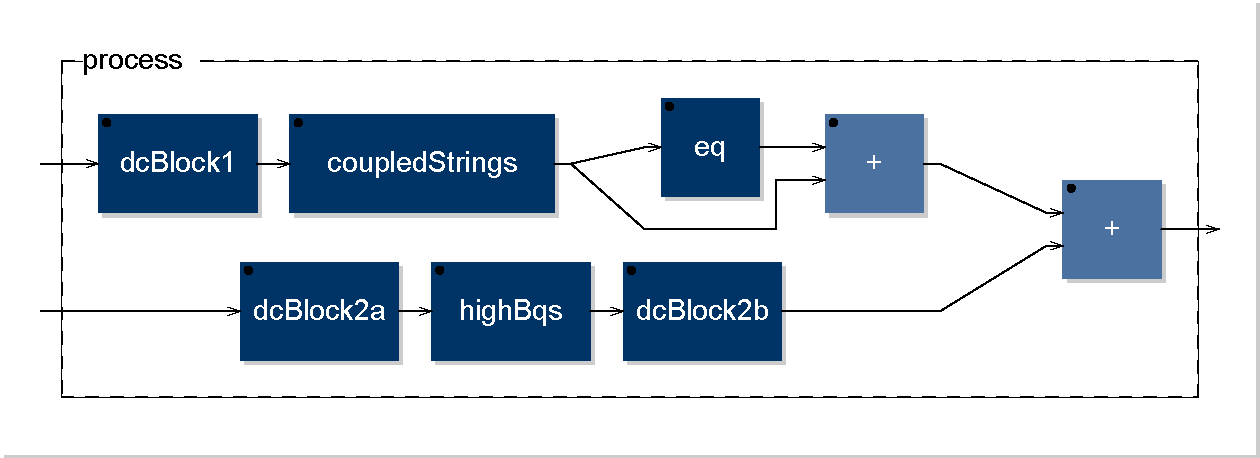
\includegraphics[width=\columnwidth]{fig/piano2.pdf}}
\caption{{\it Commuted piano algorithm drawn by FAUST using
    faust2svg. The upper figure is the beginning of the model and the
    lower figure the end.}}
\label{fig:piano}
\end{center}
\end{figure}

A commuted harpsichord has also been implemented in the {\it FAUST-STK}. It
was inspired by another {\it SynthBuilder} patch that uses a very
similar algorithm to the one described above. 

The current FAUST versions of the commuted piano and harpsichord is not a polyphonic
instrument. However, the {\it faust2pd} program developed by Albert
Graef \cite{faust2pd} makes it possible to automatically produce {\it PureData}
patches that implement polyphonic synthesizers that use FAUST generated
PD plug-ins. They can then be controlled via MIDI or OSC directly in
PureData.    

\begin{figure}[ht]
\begin{center}
        \framebox{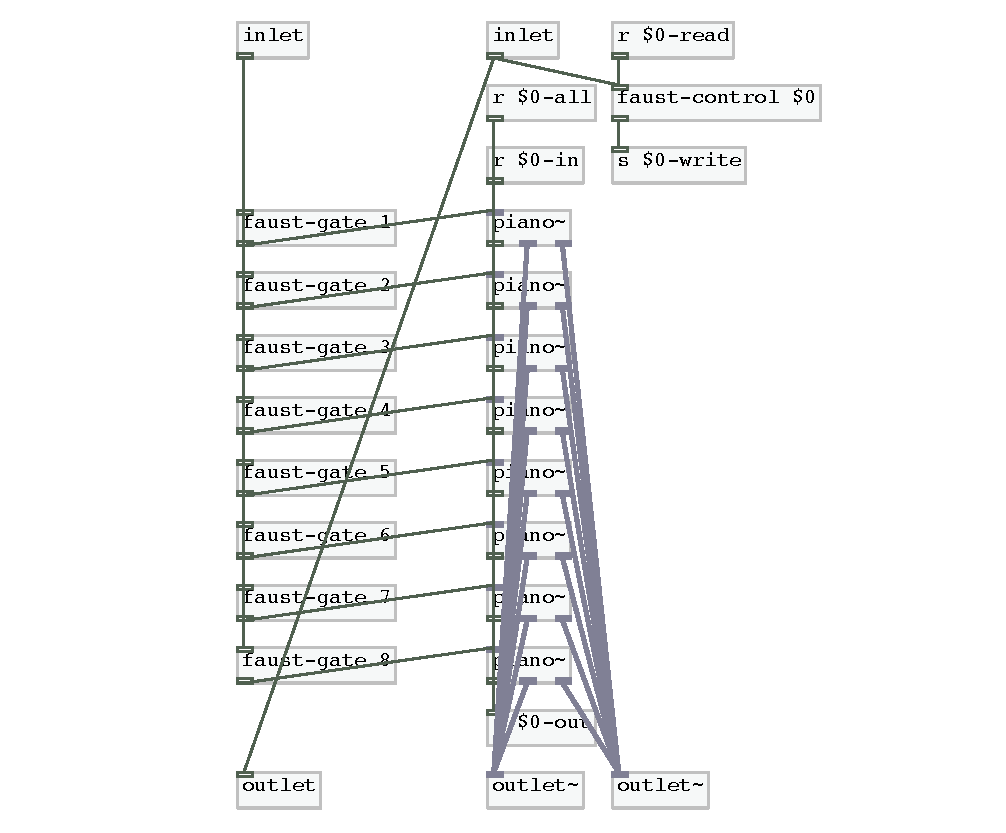
\includegraphics[width=\columnwidth]{fig/pianoPatch.pdf}}
\caption{{\it Synthesis part of the PureData polyphonic sub-patch
    generated with faust2pd from ``piano.dsp''. In the current case, a
  height voices polyphony synthesizer is implemented so
  piano$\sim$.dsp is called height times.}}
\label{fig:pianoPatch}
\end{center}
\end{figure}

\section{Using a FAUST-STK physical model with gesture following
  datas}

Parameter values are very important when dealing with physical
modeling. Indeed, even if in most cases it is possible to produce nice
sounds with static values for each parameter, the sound quality can be
improved a lot by using dynamic values that can describe better the state
of the model in function of the note and the amplitude being played.

E. Maestre worked during his phd on modeling the instrumental gesture
for the violin \cite{Esteban} at the MTG\footnote{Music Technology
  Group, University Pompeu Fabra, Barcelona (Spain).}. With his help,
it was possible to modify the algorithm of the bowed instrument from
the {\it STK} in order to make it compatible to
gesture datas. The following changes were performed on the model:
\begin{itemize}
\item the {\it ADSR} used to control the bow velocity was removed;
\item a ``force'' parameter that control the slope of the bow table
  was added;
\item a switch was added at the output of the bow table;
\item we created a four strings violin where it is possible to modify
  the value of the parameters of each string independently;
\item the simple body filter was replaced by a bank of biquad filters that apply
  a violin impulse response on the generated sound
\item an improved reflexion filter also based on a bank of
  biquad is used.  
\end{itemize}

The FAUST code was used to create a {\it PureData} plug-in. The gesture datas for
each physical parameter (note frequencies, bow position, bow velocity,
bow force and number of the string to be used) of the violin model
were placed in separated text files that can be used in a {\it PD} patch. In
the example shown in figure \ref{fig:subPatchViolin}, the values are
changed every 4.167 milliseconds. The gesture datas used plays a
traditional spanish song called Mui�eira.     

\begin{figure}[ht]
\begin{center}
        \framebox{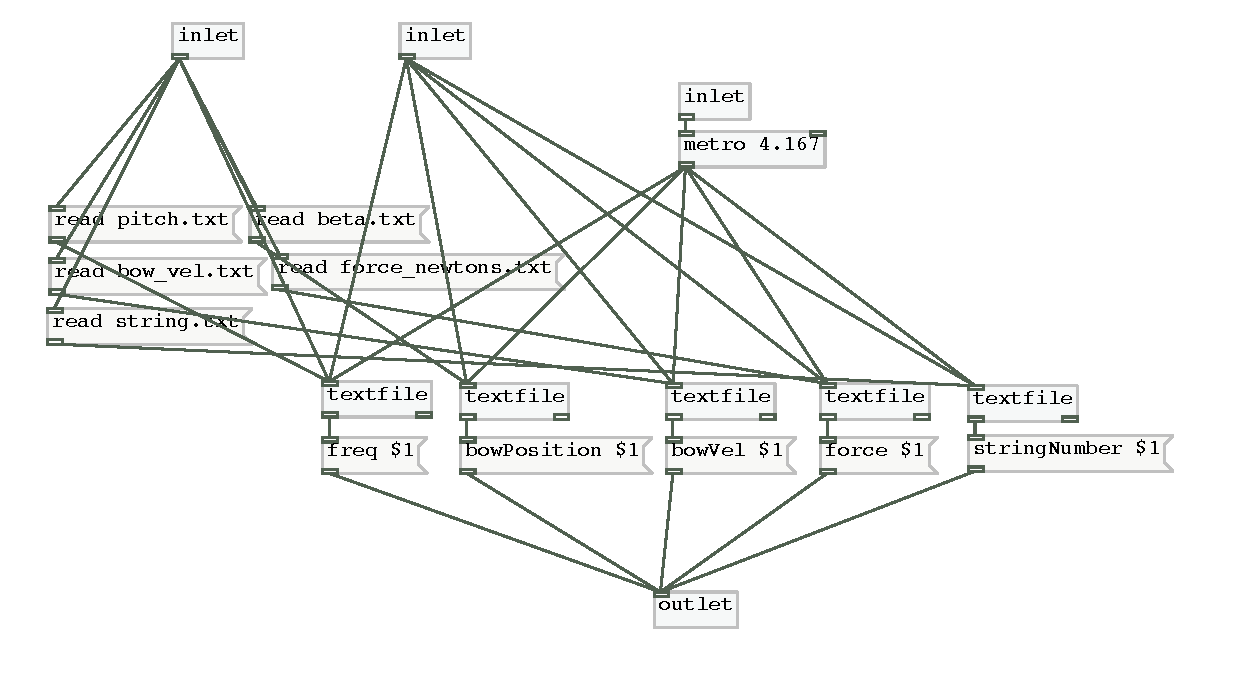
\includegraphics[width=\columnwidth]{fig/subPatchViolin.pdf}}
\caption{{\it PureData sub-patch used to send the gesture datas of
    Mui�eira in the FAUST generated plug-in.}}
\label{fig:subPatchViolin}
\end{center}
\end{figure}

\section{Optimization and Performances}

\subsection{File size}

Digital signal processing algorithms can be expressed very shortly in
FAUST. The gain in term of code size with C++ or even matlab
implementations is most of the time very significant. Thereby, we tried
to make the {\it FAUST-STK} algorithms as concise and readable as
possible.

It would be very hard and inaccurate to compare the raw C++ and
FAUST codes together as most of the physical models were implemented
in the {\it Synthesis ToolKit} with several spread out functions that
are most of the time strewn in different files. Moreover, these
functions also contains informations that are not related to the
algorithm itself.

Nevertheless, we were able to carry out such a comparison as a rough
guide. We took into account in FAUST as in C++ the implementation of the
algorithm itself and the line concerning parameters
handling. 

The result of this comparison can be seen in table \ref{tab:nblines}. Once again, even if its results are certainly arguable, it
shows very well how FAUST is efficient in reducing the code
size. 

\begin{table*}[ht]
\begin{center}
\begin{tabular}{c c c c c c c}
\hline
\hline
FAUST file & C++ code & FAUST code & Size gain for & C++ code & FAUST code
& Size gain for\\
name & nb of declarations & nb of declarations & nb of lines & nb of lines & nb of
lines & nb of lines\\
\hline
blowBottle.dsp  & 74 & 30 & {\bf 59.5\%} & 237 & 54 & {\bf 77.2\%} \\
blowHole.dsp & 131 & 66 & {\bf 49.6\%} & 373 & 104 & {\bf 72.1 \%} \\
bowed.dsp &  92 & 45 & {\bf 51.1\%} & 274 & 69 & {\bf 74.8\%} \\
brass.dsp & 90 & 36 & {\bf 60\%} & 272 & 63 & {\bf 76.8\%} \\
clarinet.dsp & 78 & 35 & {\bf 55.1\%} & 255 & 60 & {\bf 76.5\%} \\
flutestk.dsp & 109 & 43 & {\bf 60.6\%} & 309 & 70 & {\bf 77.3\%} \\
modalBar.dsp * & 63 & 37 & {\bf 42.3\%} & 217 & 78 & {\bf 64\%} \\
saxophony.dsp & 98 & 42 & {\bf 57.1\%} & 308 & 69 & {\bf 77.6\%} \\
sitar.dsp & 57 & 25 & {\bf 56.1\%} & 193 & 42 & {\bf 78.2\%} \\
bars * & 164 & 35 & {\bf 78.7\%} & 396 & 70 & {\bf 82.3\%} \\
voiceForm.dsp * & 121 & 65 & {\bf 46.3\%} & 325 & 109 & {\bf 66.5\%} \\
piano.dsp * & 292 & 158 & {\bf 45.9\%} & 750 & 246 & {\bf 67.2\%} \\
\hline
\end{tabular}
\end{center}
\caption{{\it Comparison of the code size of the STK object's C++ code
    with the FAUST code from FAUST-STK. The number of declarations was
    calculated in both cases by counting the number of semicolons in the
    code. In the case of the
    instruments where the file name is followed by the
  * sign, parameters data-bases were not taken into account.}}
\label{tab:nblines}
\end{table*}

\subsection{CPU load}

The FAUST compiler optimizes the efficiency of its generated C++
code. Thus, we tried to compare for some models the CPU load between
{\it PureData} plug-ins created using the {\it stk2pd}\footnote{{\it
    stk2pd} is a program that was developed at Stanford's
  CCRMA by M. Gurevich and C. Chafe. It converts any C++ code from the {\it
  STK} into a plug-in for {\it PureData} \cite{stk2pd}.} program with
PD plug-ins generated by FAUST using the {\it PureData} architecture
file.

In both cases, PD plug-ins were compiled in 32bits and the signal
processing is scalar. Tests were carried out on a MacBook Pro with the
following configuration:
\begin{itemize}
\item processor: 2.2 GHz Intel Core 2 Duo;
\item RAM: 2GBytes DDR2.  
\end{itemize}

Results of this comparison can be seen in table \ref{tab:computationalTest}.

\begin{table}[ht]
\begin{center}
\begin{tabular}{c c c c}
\hline
\hline
FAUST file & STK & FAUST & Difference \\
name &  \\
\hline
blowBottle.dsp  & 3,23 & 2,49 & 22,91 \\
blowHole.dsp & 2,70 & 1,75 &  35,19\\
bowed.dsp &  2,78 & 2,28 & 17,99 \\
brass.dsp & 10,15 & 2,01 & 80,20 \\
clarinet.dsp & 2,26 & 1,19 & 47,35 \\
flutestk.dsp & 2,16 & 1,13 & 47,69 \\
saxophony.dsp & 2,38 & 1,47 & 38,24 \\
sitar.dsp & 1,59 & 1,11 & 30,19 \\
tibetanBowl.dsp & 5,74 & 2,87 & 50 \\
\hline
\end{tabular}
\end{center}
\caption{{\it Comparison of the performances of PureData plug-ins
    using the STK C++ code with their FAUST generated equivalent. Values
  in the ``STK'' and ``FAUST'' columns are CPU loads in percents. The
  ``difference'' column give the gain of efficiency in percents.}} 
\label{tab:computationalTest}
\end{table}

\section{Conclusions}

Even if the primary goal of the {\it FAUST-STK} is the use of its
physical models in a musical manner, it was also built to be a
pedagogical tool. Indeed, because of its transparence and its
efficiency, the FAUST programing language is particularly
suitable for teaching digital audio signal processing. Therefore, a
clean and well commented FAUST code is probably the best way to
document the implemented instruments.

With its continually growing users community, FAUST is becoming a high quality
tool for the implementation of audio digital signal processing
algorithms. The number of filters, effects and sound synthesizers
available in FAUST is constantly increasing. The combined forces of
JACK\footnote{JACK Audio Connection Kit: \url{http://jackaudio.org}.}
and FAUST recently upgraded by the possibility to control the
generated programs with the
OSC\footnote{Open Source Control is a content format for messaging
  among computers, sound synthesizers and other multimedia devices.}
communication standard constitue a high efficiency work platform whose
limits are only constrained by the user imagination.    

\section{Acknowledgments}
This work was carried out in the frame of the ASTREE\footnote{Analyse
  et Synth�se de Traitement en Temps R�el.} project supported
by the Agence Nationale de Recherche (ANR-08-CORD-003).

%\newpage
\nocite{*}
\bibliographystyle{IEEEbib}
\bibliography{ref} % requires file template.bib

\end{document}
